\documentclass[12pt,oneside]{article}
\usepackage{makeidx,anysize,mflogo,xspace,float,epsfig,url}
\usepackage{amsmath,amsfonts,amssymb,a4wide} 
\usepackage[utf8]{inputenc}
%\usepackage[francais]{babel}
\usepackage[french]{babel}
\urlstyle{sf}
%\usepackage{subcaption}
\usepackage{hyperref}
\usepackage{graphicx}
\usepackage{graphics}
\usepackage{float}
\usepackage{caption}
\usepackage{colordvi} %??
\usepackage{listings} 
\usepackage{subfigure}
\usepackage{subfloat}
\usepackage{xcolor}
%\usepackage[labelsep=quad,indention=10pt]{subfig}
\definecolor{grey}{rgb}{0.95,0.95,0.95} % on définit la couleur grise
	% (c'est un gris très clair)
	\definecolor{red}{rgb}{1.0,0.0,0.0} 
	\definecolor{green}{rgb}{0.0,1.0,0.0}
	\definecolor{blue}{rgb}{0.0,0.0,1.0}
	\lstloadlanguages{bash,Java,C,C++,csh,make,sh}%%[Visual]Basic,xml}
	\lstset{frame=none,basicstyle=\footnotesize,breaklines,tabsize=2,captionpos=b,
		prebreak={\hbox{$\rightarrow$}},postbreak={\hbox{$\hookrightarrow$}},
		showstringspaces=false,backgroundcolor=\color{grey}\bfseries,
		keywordstyle=\color{blue},commentstyle=\color{green}\textit,
		stringstyle=\color{red}\ttfamily,abovecaptionskip=2pt,aboveskip=0pt,
		belowskip=0pt,belowcaptionskip=0pt,numbers=none,columns=fullflexible, backgroundcolor=\color{grey}}
\graphicspath{{./figures/}{./results/}}
%left,numberstyle=\footnotesize,
%		stepnumber=2,numbersep=1pt}

\begin{document}


\begin{center}
{\bf \Large Redpitaya~: Second exemple de projet Vivado ADC et DAC} \\ \ \\
G. Goavec-M\'erou, J.-M Friedt \\ \ \\ \today
\end{center}

Ce document a pour vocation de poursuivre le tutorial pr\'ec\'edent sur lequel il se base. Il
aboutit \`a non-seulement duppliquer sur DAC les mesures de l'ADC, mais \`a permettre
d'acqu\'erir ces mesures sur le PS en vue de leur sauvegarde et traitement ultr\'erieur
(Fig. \ref{fin}).

\begin{figure}[h!tb]
\hspace*{-1cm}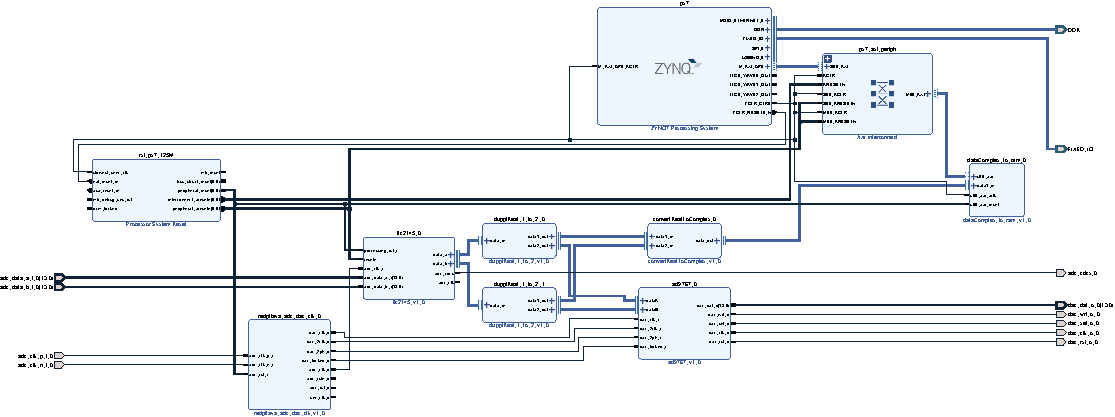
\includegraphics[width=1.2\linewidth]{design_1.pdf}
\caption{Sch\'ema final de la cha\^\i ne de traitement qui sera d\'ecrite dans ce document}
\label{fin}
\end{figure}

\section{Envoi des donn\'ees vers le PS~: c\^ot\'e PL}

Transf\'erer les donn\'ees de l'ADC vers le PS en plus d'aller vers le DAC
n\'ecessite d'une part de duppliquer les flux de donn\'ees, et de combiner
les deux voies en un flux interlac\'e de donn\'ees.

Pour ce faire~:
\begin{enumerate}
\item ajouter {\tt dupplReal\_1\_to\_2}, {\tt convert\_2x16\_to\_1\_16} (conversion de 
deux flux r\'eels vers un complexe) puis {\tt data16Complex\_to\_RAM}
\item Double clicker sur {\tt dupplReal\_1\_to\_2} et passer en 14 bits (reproduire
pour les deux doubleurs de flux). Idem pour {Convert\_2x16\_to\_1\_16}
\item Relier {\tt Data1\_out} de chaque {\tt dupplReal} vers {\tt data1\_in} et 
{\tt data2\_in} respectivement de {\tt Convert\_2x16\_to\_1\_16}
\item Couper les fils entre ADC et DAC, et passer par les deux sorties libres des
{\tt dupplReal\_1\_to\_2} 
\item Connecter {\tt data\_a} et {\tt data\_b} de l'ADC sur les deux entr\'ees libres 
des {\tt dupplReal\_1\_to\_2}
\item {\tt data16Complex\_to\_RAM}~: passer {\tt Data Size} en 14 bits et 
{\tt Addr Size} en $log_2$ du nombre d'\'echantillons voulus. En donnant 12~bits de
taille d'adresse, nous d\'efinissons {\bf 4096 couples d'\'echantillons} (complexes) 
cod\'es chacun sur 16~bits soient 16384~octets \`a transf\'erer vers le PS.
\end{enumerate}

Une fois ces blocs d\'efinis, ex\'ecuter {\tt Run Connection Automation} pour la 
connexion au bus AXI. 

\section{Envoi des donn\'ees vers le PS~: c\^ot\'e noyau Linux}

Le pilote qui sera n\'ecessaire pour obtenir les \'echantillons sur le PS depuis Linux 
sera {\tt data16Complex\_to\_ram\_core}. Pour le compiler, on pensera \`a exporter les 
variables

\begin{verbatim}
export BOARD_NAME=redpitaya
export BR_DIR=${HOME}/buildroot-2018.08.1/
\end{verbatim}

La compilation se fait trivialement depuis le r\'epertoire {\tt 
fpga\_driver/data16Complex\_to\_ram\_core}. Dans le contexte d'un {\em devicetree overlay},
nous ne chargerons par explicitement le bitstream (FPGA) et le module noyau, mais demanderons
au devicetree d'effectuer le travail pour nous. Le greffon au devicetree se g\'en\`ere gr\^ace
\`a un outil nomm\'e {\tt module\_generator} dans {\tt fpga\_app/tools/module\_generator}
con\c cu pour obtenir sa configuration depuis un fichier XML. Dans notre cas, ce fichier est
de la forme

\begin{verbatim}
<?xml version="1.0" encoding="utf-8"?>
<drivers name="design_1" version="1.0">
        <driver name ="data16Complex_to_ram" >
                <board_driver name="data1600" id = "0"
                        base_addr="0x43c00000" addr_size="0xffff" />
        </driver>
</drivers>
\end{verbatim}

avec la balise {\tt name} comportant le nom du bitstream sans son extension ni la partie
``\_wrapper'' de son nom (on notera que par d\'efaut, {\tt project\_1} est le nom propos\'e
par Vivado pour g\'en\'erer {\tt project\_1\_wrapper.bit.bin}). La balise {\tt driver}
renseigne du module noyau charg\'e, et {\tt base\_addr} ainsi que {\tt addr\_size}
renseignent des plages d'adresses attribu\'ees \`a l'IP tel qu'indiqu\'e par Vivado
(Fig. \ref{addr}).

\begin{figure}[h!tb]
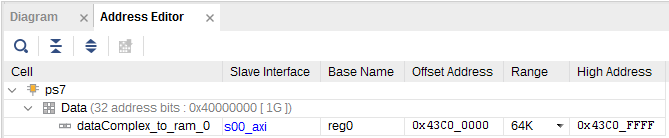
\includegraphics[width=\linewidth]{adresses}
\caption{Plage d'adresses occup\'ees par l'IP charg\'ee de communiquer sur bus AXI entre
PL et PS.}
\label{addr}
\end{figure}

Ce fichier XML est converti en greffon {\em devicetree} par\\
{\tt fpga\_app/tools/module\_generator/module\_generator -dts jmf.xml}

puis converti en binaire {\em devicetree overlay} par

\hspace*{-2.53cm}
{\footnotesize
\verb~[...]/buildroot/output/build/linux-[...]/scripts/dtc/dtc -@ -I dts -O dtb -o project_1.dtbo project_1.dts~}

\`A l'issue de cette compilation, nous avons d\'esormais trois fichiers \`a notre disposition
sur le PC que nous transf\'erons vers la Redpitaya
\begin{enumerate}
\item le bitstream au format {\tt .bit.bin}
\item le module noyau d'extension {\tt .ko}
\item le {\em devicetree overlay} d'extension {\tt .dtbo}
\end{enumerate}

\section{Sur la Redpitaya ...}

Ayant transmis ces fichiers sur la Redpitaya, le m\'ecanisme de {\em devicetree overlay}
est activ\'e de fa\c con \`a charger en coh\'erence toutes ces informations par
\begin{enumerate}
\item {\tt cp design\_1\_wrapper.bit.bin /lib/firmware/}
\item {\tt mkdir /sys/kernel/config/device-tree/overlays/jmf}
\item {\tt cat project\_1.dtbo > /sys/kernel/config/device-tree/overlays/jmf/dtbo}
\end{enumerate}

Si tout se passe bien, la LED bleue de la Redpitaya s'allume (bitstream charg\'e dans le FPGA)
et le module noyau est charg\'e. Il reste \`a r\'ecolter les donn\'ees par un programme trivial
de la forme

\begin{lstlisting}[language=C]
#include <stdio.h>
#include <stdint.h>
#include <fcntl.h>
#include <unistd.h>

int main()
{int k,fi,fo; char c[16384];
 fi=open("/dev/data1600",O_RDWR); fo=open("/tmp/data.bin",O_WRONLY|O_CREAT);
 for (k=1;k<5;k++) {read(fi,c,16384); write(fo,c,16384); }
 close(fi); close(fo);
}
\end{lstlisting}

dont l'ex\'ecution g\'en\`ere le fichier de points qui se lisent sous GNU/Octave par
\begin{lstlisting}[language=Octave]
f=fopen('data.bin')
d=fread(f,inf,'int16');
plot(d(2:2:end));
\end{lstlisting}

pour donner comme r\'esultat la Fig. \ref{adc} dans lequel l'entr\'ee de l'ADC est
directement connect\'ee \`a l'amplificateur non-diff\'erentiel vers diff\'erentiel
pour permettre l'exploitation volontaire du repliement spectral.

\begin{figure}[h!tb]
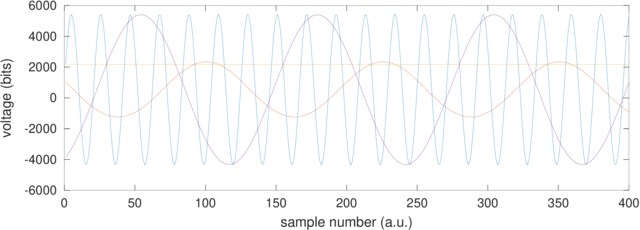
\includegraphics[width=\linewidth]{mesures}
\caption{Acquisitions issues du FPGA par le programme utilisateur communiquant avec
le noyau au travers de {\tt /dev/data1600}.}
\label{adc}
\end{figure}
\end{document}
